\section{Results}

\subsection{Core Feature Screenshots / GIFs}
This section provides visual evidence of the working application (Flask WebUI for RAG\_Core).

\begin{figure}[h]
\centering
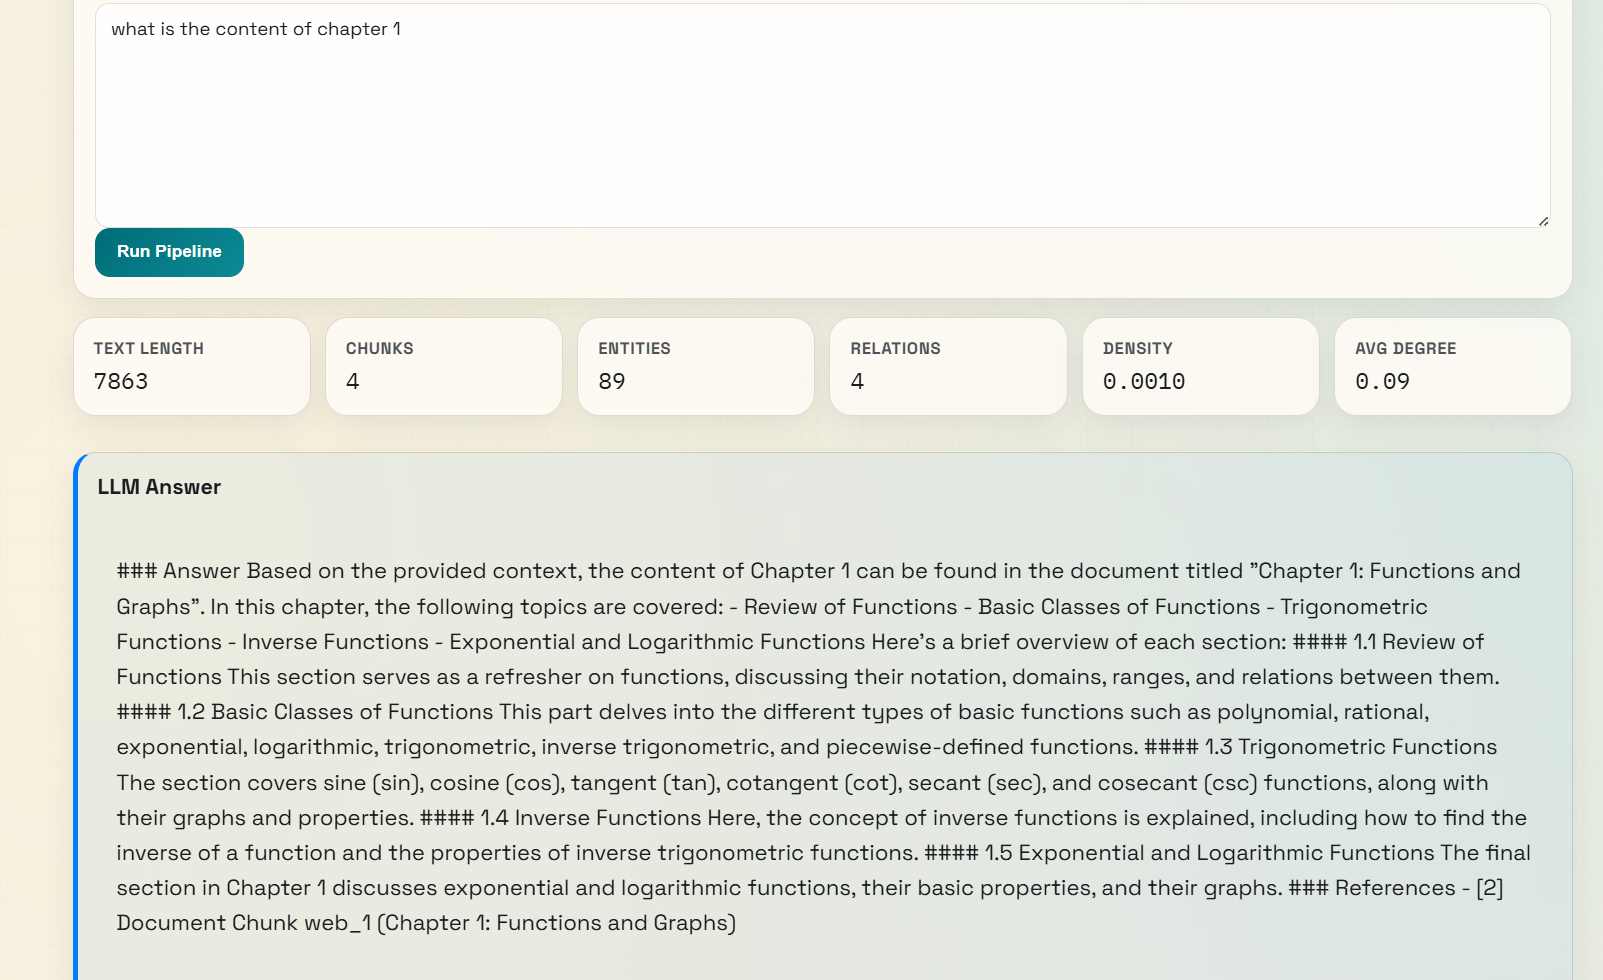
\includegraphics[width=0.95\textwidth]{Images/rag_core_webui_llm_answer.png}
\caption{RAG\_Core WebUI: running the pipeline and viewing a grounded LLM answer with graph statistics (chunks, entities, relations, density, average degree).}
\end{figure}

\subsection{UI-to-Database Mapping Analysis}
The WebUI actions map directly to property-graph operations:
\begin{itemize}
	\item \textbf{Upload/Paste Document $\rightarrow$ Chunk Nodes:} when the user uploads a file or pastes text, the backend converts it to text, then applies overlapping chunking. Each chunk carries metadata (token count, order index, file path). In a persistent graph DB, this corresponds to creating \texttt{:Chunk} nodes.
	\item \textbf{Run Pipeline $\rightarrow$ Upsert Entities/Edges:} entity and relation extraction produces candidates per chunk. The backend upserts \texttt{:Entity} nodes and \texttt{:RELATED\_TO} relationships, merging duplicates and accumulating weights across mentions.
	\item \textbf{Keyword Query $\rightarrow$ Graph Index/Search:} the \textit{Keyword Query} field triggers an entity keyword search over node names/descriptions (prototype uses token overlap scoring; Neo4j can use a full-text index).
	\item \textbf{Entity Query $\rightarrow$ Neighborhood Expansion:} the \textit{Entity Query} field triggers a depth-limited traversal (BFS) to retrieve the entity neighborhood (1--2 hops) for local reasoning.
	\item \textbf{Natural-Language Question $\rightarrow$ Hybrid Retrieval + LLM:} the \textit{Natural Language Question} triggers translation (optional), hybrid retrieval (local + global candidates), structured context assembly (JSON blocks), and final answer generation by the LLM.
\end{itemize}

\subsection{Performance Evaluation}
We evaluate response time for core retrieval operations (micro-benchmarks). The goal is to validate that graph-oriented retrieval stays interactive as the number of entities and relations grows.

\textbf{Benchmark setup (prototype):}
\begin{itemize}
	\item Chunking: fixed token window with overlap.
	\item Extraction: mock extractor (deterministic, no external LLM calls) to isolate database/retrieval cost.
	\item Storage: in-memory property graph (Python dicts) that mirrors a Neo4j-style model.
	\item Metric: wall-clock latency (ms), averaged over repeated runs.
\end{itemize}

\begin{table}[h]
\centering
\begin{tabular}{|c|c|c|c|c|c|c|}
\hline
\textbf{Scale} & \textbf{Chunks} & \textbf{Nodes} & \textbf{Edges} & \textbf{Build graph (ms)} & \textbf{Keyword search (ms)} & \textbf{Neighborhood (ms)} \\
\hline
Small & 20 & 1000 & 20 & 3.21 & 0.52 & 0.01 \\
\hline
Medium & 100 & 5000 & 100 & 24.79 & 2.63 & 0.01 \\
\hline
Large & 400 & 20000 & 400 & 95.38 & 10.49 & 0.05 \\
\hline
\end{tabular}
\caption{Micro-benchmark results (average over 5 runs) using mock extraction and the in-memory property graph. Values vary by hardware and configuration.}
\end{table}

The benchmarks demonstrate that neighborhood traversal and keyword search remain fast for interactive usage in the prototype. For production-scale datasets, we would persist the graph in Neo4j and rely on native indexing and optimized traversal execution.